\begin{frame}
    \vspace*{1.3in}
    \begin{center}
        \Large \textbf{Conclusions}: Current and Future Work
    \end{center}
\end{frame}

\begin{frame}{\small Conclusions and Future Work}
    \vspace*{-0.2in}
    \footnotesize
    \begin{columns}
        \begin{column}{0.6\textwidth}
            \only<1>{
                \begin{figure}
                    \centering
                    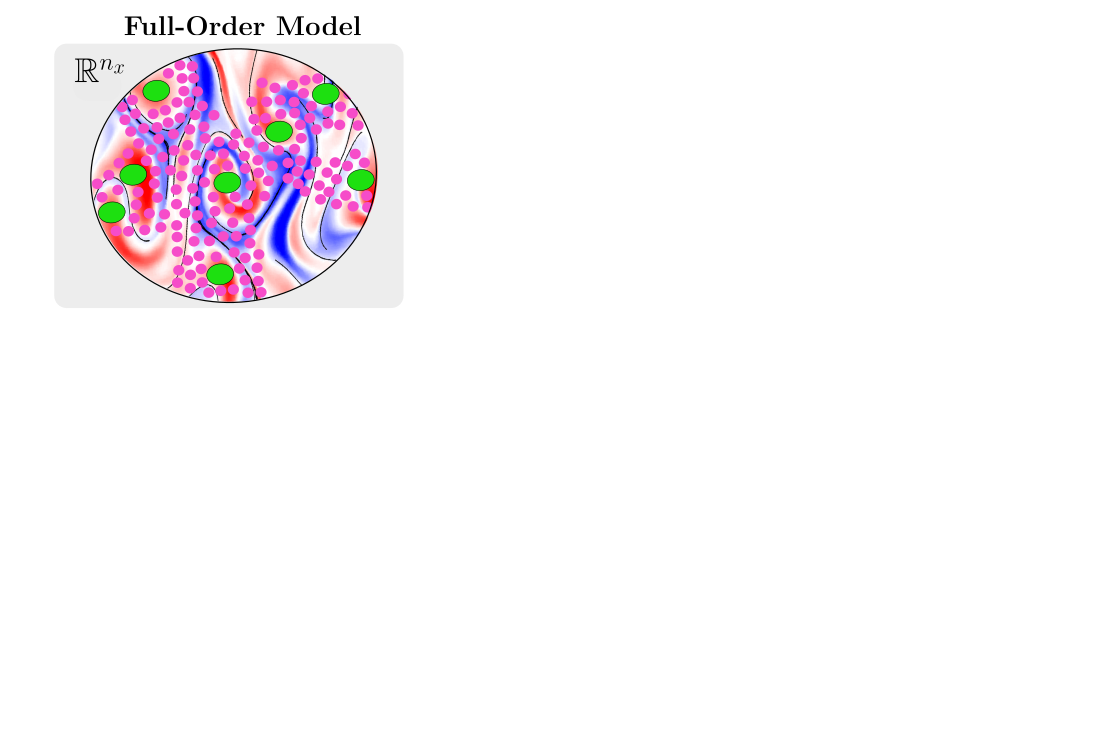
\includegraphics[width=0.99\textwidth]{../figs/conclusions/conclusion_overview_1.png}
                \end{figure}}
            \only<2>{
                \begin{figure}
                    \centering
                    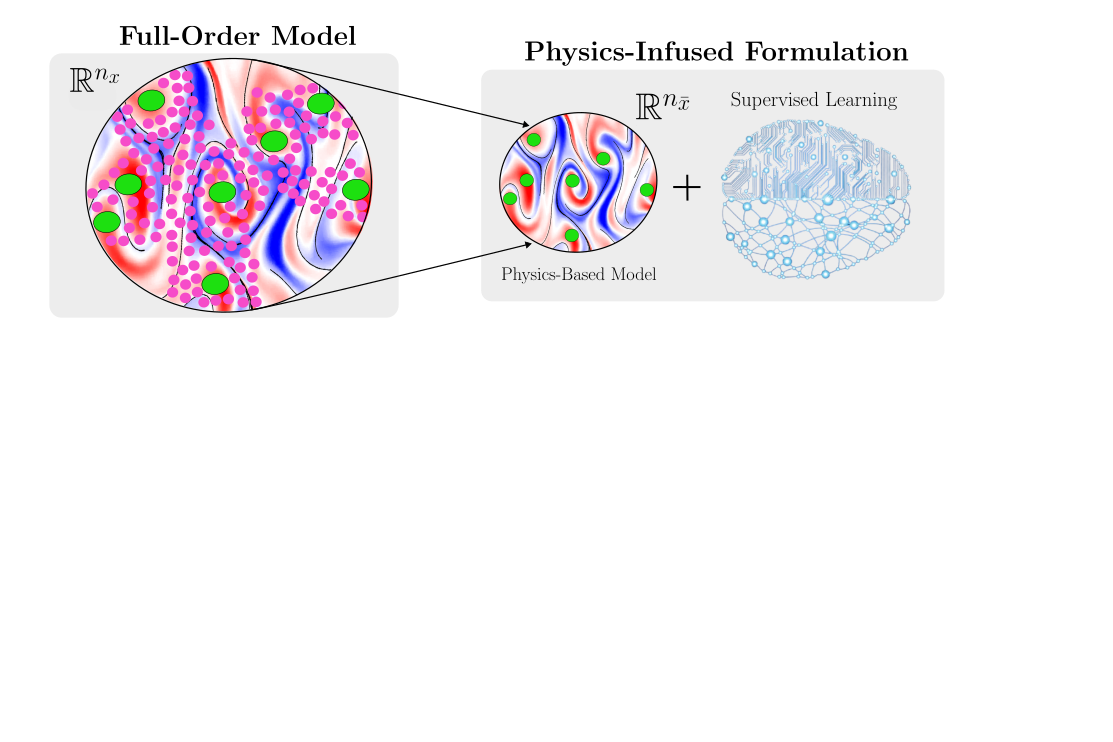
\includegraphics[width=0.99\textwidth]{../figs/conclusions/conclusion_overview_2.png}
                \end{figure}}
            \only<3>{
                \begin{figure}
                    \centering
                    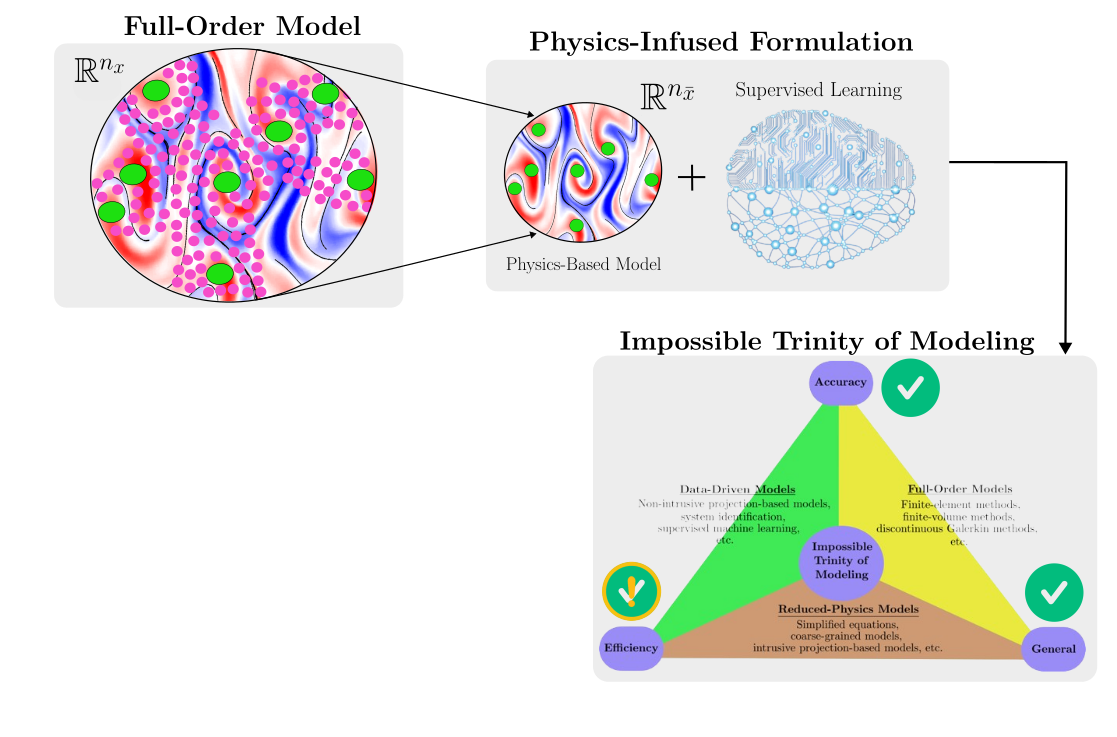
\includegraphics[width=0.99\textwidth]{../figs/conclusions/conclusion_overview_3.png}
                \end{figure}}
            \only<4>{
                \begin{figure}
                    \centering
                    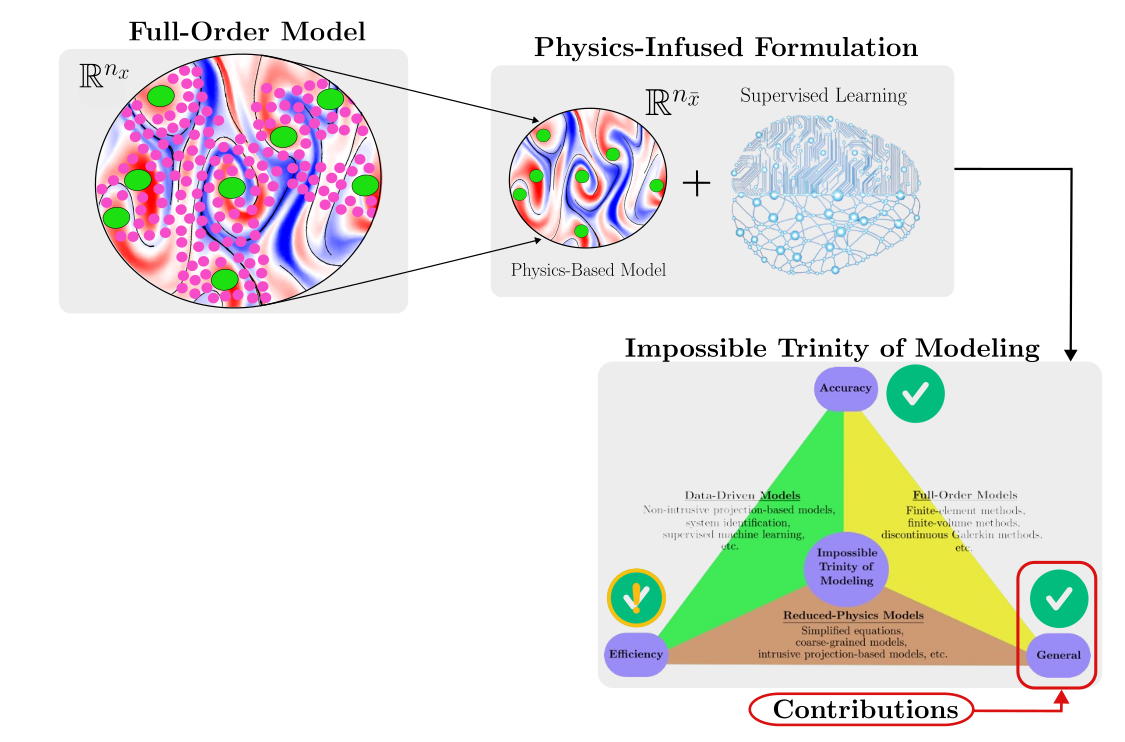
\includegraphics[width=0.99\textwidth]{../figs/conclusions/conclusion_overview_4.png}
                \end{figure}}
            \only<5>{
                \begin{figure}
                    \centering
                    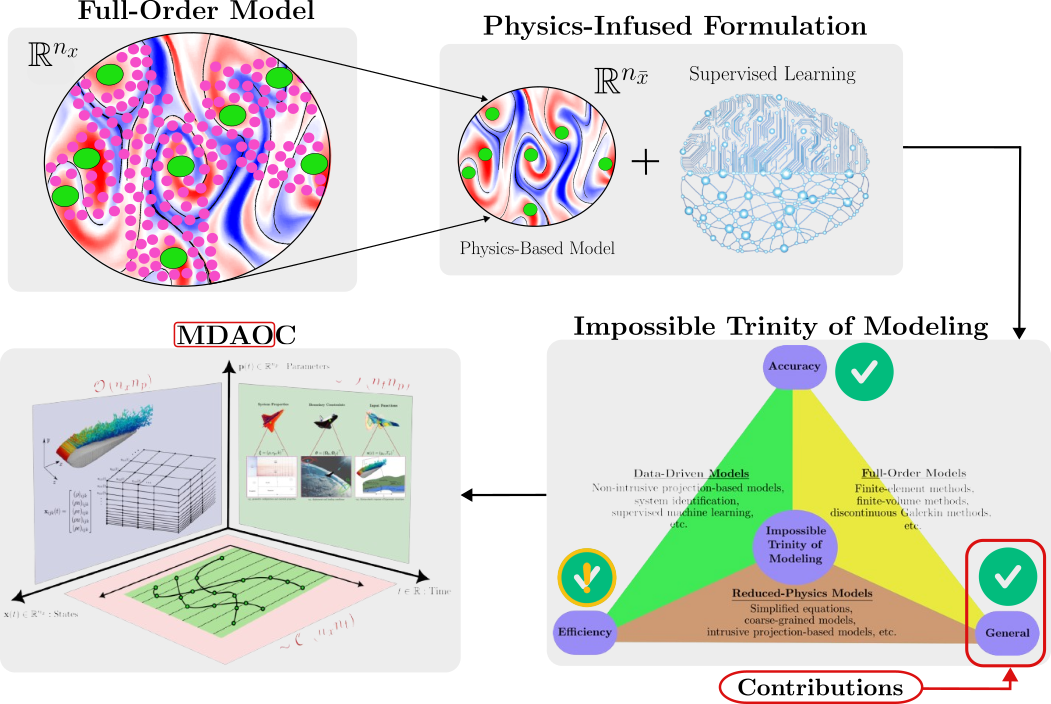
\includegraphics[width=0.99\textwidth]{../figs/conclusions/conclusion_overview_5.png}
                \end{figure}}
            \only<6->{
                \begin{figure}
                    \centering
                    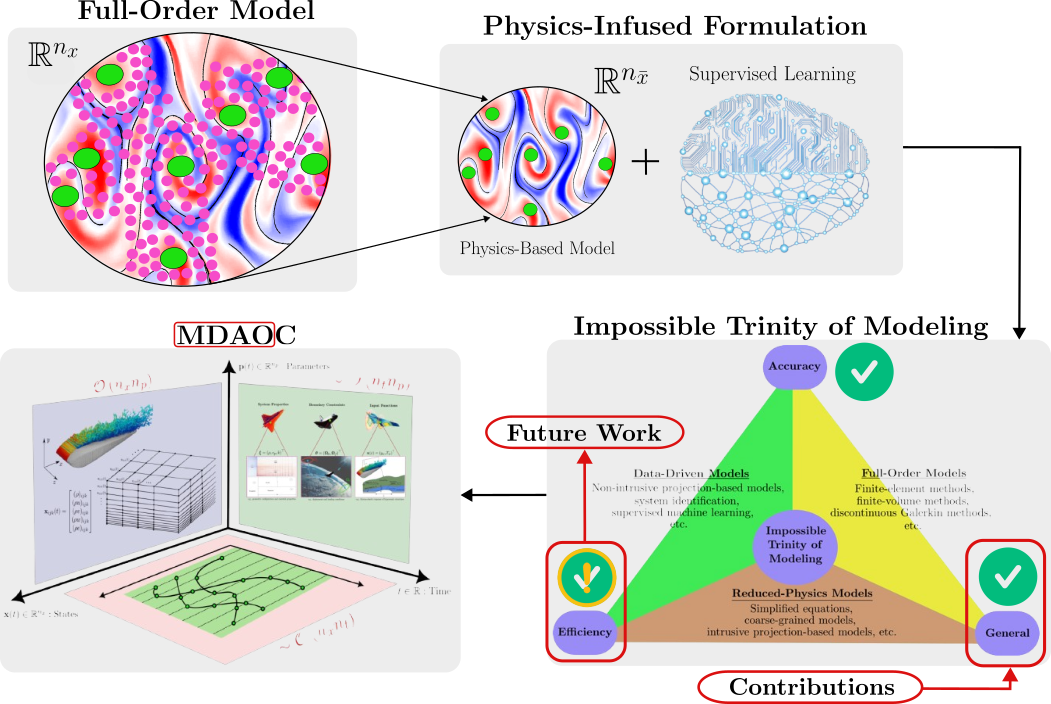
\includegraphics[width=0.99\textwidth]{../figs/conclusions/conclusion_overview_6.png}
                \end{figure}}
        \end{column}
        \begin{column}{0.4\textwidth}
            \tiny
            \visible<4->{
                \begin{center}
                    \textbf{Main Advantages}
                \end{center}
                \vspace*{-0.1in}
                \begin{itemize}
                    \item \textcolor{red}{\textbf{Systematic approach}} to physics infusion
                    \item Improved \textcolor{red}{\textbf{generalizability}}
                \end{itemize}}
            \visible<6->{
            \begin{center}
                \textbf{Current and Future Work}
            \end{center}
            \vspace*{-0.1in}
                \begin{itemize}
                    \item<7-> Training overheads are still large \textcolor{red}{\textbf{(similar to neural ODE)}},
                    \item<8-> \textcolor{red}{\textbf{Learning from sparse noisy observables}} (on-going work),
                    \item<9> \textcolor{red}{\textbf{Apply PIROM to more complex multi-physical settings}} (e.g., on-going work on ablating hypersonic TPS).
                \end{itemize}}
        \end{column}
    \end{columns}
\end{frame}

\begin{frame}
    \footnotesize
    \vspace*{1.3in}
    \begin{center}
    \Huge
    Thank You! Questions?\\
    \underline{\textcolor{blue}{cavarga@sandia.gov}}
    \end{center}
\end{frame}